\chapter{Wyniki}

\section{Baza danych}
-znaczenie danych

\section{Sekwencje ogórka}
\todo{tabela z wynikami \ref{tab:genome_stat}}

\begin{table}
	\centering
	\begin{tabular}{|c||r|r|r|c|} \hline
		\textbf{Chromosom}    & Długość [Mbp] & Liczba & Zmapowana & Zmapowana \\
		& & zmapowanych contigów & długość [bp] & długość [\%] \\
		\hline
		\textbf{1}             & 55                 &  22                 &  32970425          & 59.9\%               \\
		\textbf{2}             & 44                 &  13                 &  23992470          & 52.2\%               \\
		\textbf{3}             & 65                 &  14                 &  39532546          & 60.8\%               \\
		\textbf{4}             & 61                 &  15                 &  24781874          & 40.6\%               \\
		\textbf{5}             & 49                 &  22                 &  26573846          & 54.2\%               \\
		\textbf{6}             & 42                 &  19                 &  29507078          & 70.2\%               \\
		\textbf{7}             & 52                 &  11                 &  18951584          & 36.4\%               \\
		\hline
		$\mathbf{\Sigma}$      &368                 & 116                 & 196309823          &  53.3\%              \\
		\hline
	\end{tabular}
	\caption{Chromosome statistic for mapped contigs of Nothern European cucumber genome.
		The length of the chromosomes and length of the genome described in~Chen's studies\cite{article:reevaluation_in_cucumber} was used.}
	\label{tab:genome_stat}
\end{table}

\section{API}

\section{Algorytmy}
Porównanie ze sobą dwóch sekwencji nie może polegać na zwykłej analizie ciągów tekstowych, ponieważ porównując ciągi musimy brać pod uwagę ich podłoże ewolucyjne. Chcemy sprawdzić na ile podobna jest jedna sekwencja do drugiej, analizując możliwość ewolucyjnego przekształcenia pierwszej w drugą. 
\todo{porównanie, komentarz}

\begin{figure}[h]
	\centering
	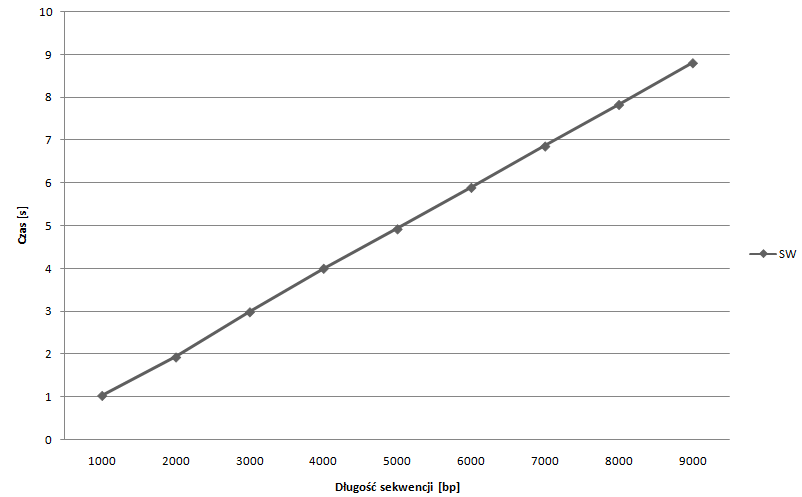
\includegraphics[width=1\textwidth]{img/sm-sekwencja-zmienna.png}
	\caption{\todo{opis - zmienna sekwencja}}
	\label{img:sm-sekwencja-zmienna}
\end{figure}

\begin{figure}[h]
	\centering
	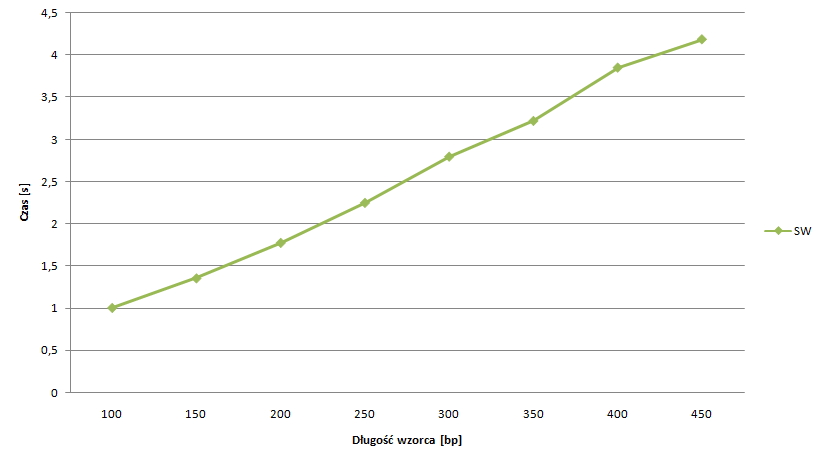
\includegraphics[width=1\textwidth]{img/sm-wzorzec-zmienny.png}
	\caption{\todo{opis - zmienny wzorzec}}
	\label{img:sm-wzorzec-zmienny}
\end{figure}

\begin{figure}[h]
	\centering
	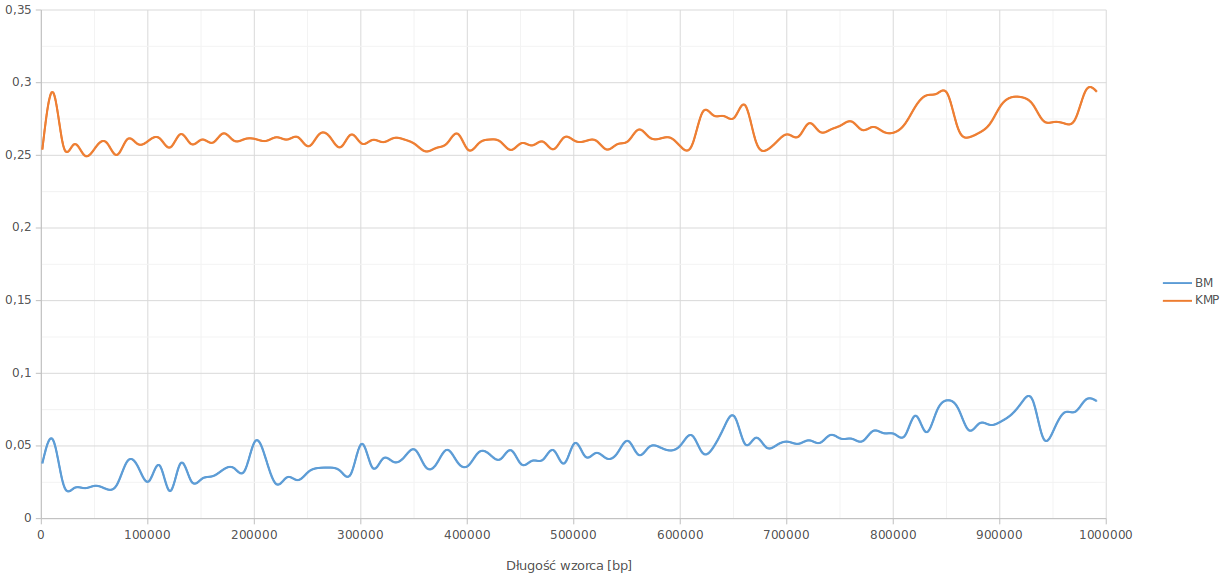
\includegraphics[width=1\textwidth]{img/kmp-vs-bm.png}
	\caption{\todo{opis - BMP vs KMP}}
	\label{img:kmp-vs-bm}
\end{figure}